\documentclass[conference]{IEEEtran}
\IEEEoverridecommandlockouts
% The preceding line is only needed to identify funding in the first footnote. If that is unneeded, please comment it out.
\usepackage{cite}
\usepackage{amsmath,amssymb,amsfonts}
\usepackage{algorithmic}
\usepackage{graphicx}
\usepackage{textcomp}
\usepackage{xcolor}
\def\BibTeX{{\rm B\kern-.05em{\sc i\kern-.025em b}\kern-.08em
    T\kern-.1667em\lower.7ex\hbox{E}\kern-.125emX}}
\begin{document}

\title{Playing Atari Games using Deep Reinforcement Learning\\}

\author{\IEEEauthorblockN{Nihesh Anderson}
\IEEEauthorblockA{\textit{Undergraduate (CSE Dept)} \\
\textit{IIIT Delhi}\\
Delhi, India \\
nihesh16059@iiitd.ac.in}
\and
\IEEEauthorblockN{Arushi Chauhan}
\IEEEauthorblockA{\textit{Undergraduate (CSE Dept)} \\
\textit{IIIT Delhi}\\
Delhi, India \\
arushi16019@iiitd.ac.in}
}

\maketitle

\begin{abstract}
In this intermediate report, we will talk about different techniques used in implementing a reinfocement learning agent for playing Atari games. This project is inspired by the paper "Playing Atari with Deep Reinforcement Learning" by V. Minh, et. al. This report contains a summary of the work done so far, and the plan for the second half of the project timeline. 
\end{abstract}

\begin{IEEEkeywords}
Reinforcement Learning, Atari, Q learning
\end{IEEEkeywords}

\section{Introduction}
This report describes the use of Q learning model and Deep CNNs for building a reinforcement learning agent for playing Atari games. We also talk about the results obtained so far, along with a brief idea about why we got those numbers and possible remedies to improve them. 

\section{Implementation} 
\subsection{Deep Q Network architecture}
In our model, we have used the following layers:
\begin{itemize}
\item Convolutional layer with 8x8 filter, 4x4 stride.
\item Convolutional layer with 4x4 filter, 2x2 stride.
\item Convolutional layer with 3x3 filter, 1x1 stride.
\item Dense layer with 512 neurons and relu activation
\item Dense layer with neurons equal to the number of actions to predict the Q function for different actions.
\item All the layers use relu activation. 
\end{itemize}
\subsection{Preprocessing and Experience Replay}
Every frame of the game is reduced to $84 \times 110$ so that unwanted pixels are removed. Also, the image is converted to grayscale as there is no loss of information by doing so. Training based on the most recent experiences may lead to learning a biased model. Hence, we store the set of experiences/history in a deque and randomly choose a mini batch from this pool of experiences for training. This ensures that the model learns a wide range of strategies. 
\subsection{Double DQN}
The Q function is a recursively defined function. Updating Q values based on the values returned by the CNN might lead to a lot of oscillations and the Q function might take a lot of time to converge to the actual Q function. Hence, we use two networks; the learner and the predictor. Predictor remains constant over a period of time and feeds the Q value of the next state to the learner so that there is a notion of stable learning, in case of the learner. Periodically, the predictor's weights is updated to the learner's weights. 
\subsection{Exploration vs Exploitation}
Whenever the agent has to play a move, it performs a random action with a probability of $\epsilon$. The value of $\epsilon$ is set to 1 initially, and it is annealed at a constant rate down to a small value. This is done so that there's a lot of exploration in the initial phase of learning and exploitation as the model's knowledge enhances. 
\section{Results}
\begin{center}
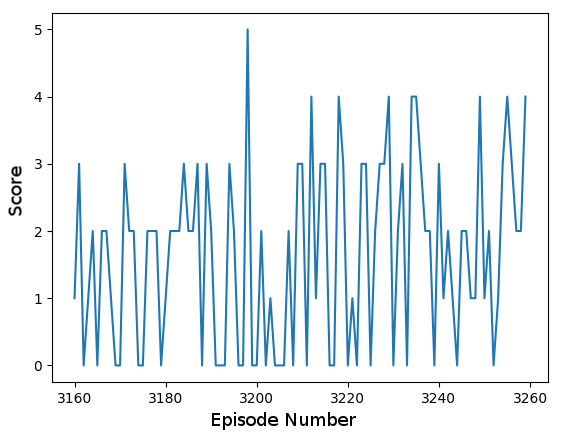
\includegraphics[scale=0.3]{Result.png}
\end{center}
After training for over 3500 episodes (equivalent to 10 hours), the model could reach an average score of 1.5 per episode. Although it is performing better than making random moves, this score is certainly far from what has been achieved in the paper. 
\section{Future Work}
So far, we have been on par with the timeline, except the last phase where training and parameter tuning took more time than what we expected. In the second phase of the project, we will focus on debugging our model by changing the learning parameters in order to improve performance. It is known that the actual state of the art results were obtained on high performance computers. Due to lack of computational resources, we will have to restrict the size of replay memory, thereby capping the performance at a slightly lower level.  

\begin{thebibliography}{00}
\bibitem{b1} V. Minh, K. Kavukcuoglu, D. Silver, A. Graves, I. Antonoglou, D. Wierstra, M. Riedmiller Playing Atari with Deep Reinforcement Learning, NIPS 2013.
\end{thebibliography}
\end{document}
